\documentclass[12pt,a4paper]{article} %report has annoying numbering habits
\usepackage{mystyle}
\usepackage{graphicx}
\usepackage{minted}
\usepackage{listings}
\usepackage[margin=1in]{geometry}
\usepackage{pdflscape}
\usepackage{float}
\usepackage{flafter}
%\usemintedstyle{monokai}
\usepackage{auto-pst-pdf}

\title{Homework 2 - Corrected}
\author{Andrea Yocom}
 
\begin{document}
 
\maketitle	
\tableofcontents
% \listoffigures
% \listoftables

%use \input to include chapters from ./src as shown. Files can be .txt or .tex:
\section{Instructions}
\documentclass[12pt,a4paper]{article} %report has annoying numbering habits
\usepackage{mystyle}
\usepackage{graphicx}
\usepackage{minted}
\usepackage{listings}
\usepackage[margin=1in]{geometry}
\usepackage{pdflscape}
\usepackage{float}
\usepackage{flafter}
%\usemintedstyle{monokai}
\usepackage{auto-pst-pdf}

\title{Homework 2 - Corrected}
\author{Andrea Yocom}
 
\begin{document}
 
\maketitle	
\tableofcontents
% \listoffigures
% \listoftables

%use \input to include chapters from ./src as shown. Files can be .txt or .tex:
\section{Instructions}
\documentclass[12pt,a4paper]{article} %report has annoying numbering habits
\usepackage{mystyle}
\usepackage{graphicx}
\usepackage{minted}
\usepackage{listings}
\usepackage[margin=1in]{geometry}
\usepackage{pdflscape}
\usepackage{float}
\usepackage{flafter}
%\usemintedstyle{monokai}
\usepackage{auto-pst-pdf}

\title{Homework 2 - Corrected}
\author{Andrea Yocom}
 
\begin{document}
 
\maketitle	
\tableofcontents
% \listoffigures
% \listoftables

%use \input to include chapters from ./src as shown. Files can be .txt or .tex:
\section{Instructions}
\documentclass[12pt,a4paper]{article} %report has annoying numbering habits
\usepackage{mystyle}
\usepackage{graphicx}
\usepackage{minted}
\usepackage{listings}
\usepackage[margin=1in]{geometry}
\usepackage{pdflscape}
\usepackage{float}
\usepackage{flafter}
%\usemintedstyle{monokai}
\usepackage{auto-pst-pdf}

\title{Homework 2 - Corrected}
\author{Andrea Yocom}
 
\begin{document}
 
\maketitle	
\tableofcontents
% \listoffigures
% \listoftables

%use \input to include chapters from ./src as shown. Files can be .txt or .tex:
\section{Instructions}
\input{../src/hw2.txt}
%\input{./ch/ch1.tex}

\begin{landscape}
\section{Code}
\begin{minted}{python}
import numpy as np
import scipy as sp
data = np.genfromtxt('./data/hw2.csv', delimiter = ',' , usecols = (2,3))

import matplotlib
matplotlib.use('PS')
import matplotlib.pyplot as plt

# Verbosely return std dev of the temperature given a range of years
def annual_temp_stdev(data,begin,end):
    """data must be a 2-col array of year and temp, begin and end are years to define averaging"""
    #check to make sure begin and end are within range
    if begin not in data[:,0]:
        print "Beginning year not in range " + str(data[0,0]) \
        + " to " + str(data[len(data)-1,0]) + ", try again."
    elif end not in data[:,0]:
        print "Ending year not in range " + str(data[0,0]) \
        + " to " + str(data[len(data)-1,0]) + ", try again."
    else:
        #index the begin and end years
        ibegin = begin - data[0,0]
        iend = end - data[0,0]
        
        #compute standard deviation of the temperatures in the range indicated by years
        stdev = np.std(data[ibegin:iend+1,1])
        #round
        stdev = round(stdev,3)
        
        return "Standard deviation for temperatures in years " + str(begin) \
        + " to " + str(end) + " is " + str(stdev) + " degrees Fahrenheit."

# Computes the standard deviation of the 2nd col given a range of items in the 1st col
def my_stdev(data,begin,end):
    """data must be a 2-col array, begin and end are endpoints to define averaging"""
    #check to make sure begin and end are within range
    if begin not in data[:,0]:
        print "begin not in range " + str(data[0,0]) \
        + " to " + str(data[len(data)-1,0]) + ", try again."
    elif end not in data[:,0]:
        print "end not in range " + str(data[0,0]) \
        + " to " + str(data[len(data)-1,0]) + ", try again."
    else:
        #index the begin and end points
        ibegin = begin - data[0,0]
        iend = end - data[0,0]
        
        #compute standard deviation of the data in the range indicated by [begin:end+1]
        stdev = np.std(data[ibegin:iend+1,1])
    return stdev

# Computes the mean of the 2nd col given a range of items in the 1st col
def my_mean(data,begin,end):
    """data must be a 2-col array, begin and end are endpoints to define averaging"""
    #check to make sure begin and end are within range
    if begin not in data[:,0]:
        print "begin not in range " + str(data[0,0]) \
        + " to " + str(data[len(data)-1,0]) + ", try again."
    elif end not in data[:,0]:
        print "end not in range " + str(data[0,0]) \
        + " to " + str(data[len(data)-1,0]) + ", try again."
    else:
        #index the begin and end points
        ibegin = begin - data[0,0]
        iend = end - data[0,0]
        
        #compute standard deviation of the data in the range indicated by [begin:end+1]
        datamean = np.mean(data[ibegin:iend+1,1])
    return datamean

def bin_plot(data,binsize,begin,end):
    #initialize lists to store binned averages and stdevs
    years = []
    means = []
    stdevs = []
    
    #loop in increments of binsize to populate lists, 
    #up to the last full decade (doesn't work for 2011,2012 in this vsn)
    i = 0
    while i < int(round(2012-1850,-1)):
        years.append(begin+i)
        means.append(my_mean(data,begin+i,begin+i+binsize))
        stdevs.append(my_stdev(data,begin+i,begin+i+binsize))
        i += binsize
    return [years,means,stdevs]

plotdata=bin_plot(data,10,1850,2012)

[years,means,stdevs] = plotdata

#Calibrate: report standard deviations for the years 1930 to 1960 and 1980 to 2010. 

thirtyToSixty = annual_temp_stdev(data,1930,1960)
eightyToTen = annual_temp_stdev(data,1980,2010)
#output calibration
with open('./ch/calibration.txt','w') as f:
    # printString =
    f.write(thirtyToSixty + ' ' + eightyToTen)

#plotting code borrowed from Jordan
plt.plot(years,means,'ro')
plt.errorbar(years,means,yerr=stdevs,linestyle = 'None',color='blue')
plt.xlabel('Decade')
plt.ylabel("Average Temperature")
plt.title("Average Temperature by Decade")
plt.xlim([1840,2012])
plt.ylim([57,60])
plt.savefig('./img/temp_plot')
\end{minted}
\end{landscape}

\section{Output}
\subsection{Calibration}
\paragraph{}
\input{../src/calibration.txt}

\subsection{Plot}
\begin{figure}[b]
\centering
 \includegraphics[width=\textwidth]{../img/temp_plot.ps}
\end{figure}

%\section{What I learned}
%\input{../src/hw2_learn.txt}
%
% Bibliography:
% \clearpage
% \addcontentsline{toc}{chapter}{Bibliography}
% \input{./src/bibliography.tex}
 
%\appendix
%\section{Calculating the Steinhart-Hart Parameters}
%\label{parameters}
%\includepdf[pages=-]{./img/parameters}

\end{document}
%\input{./ch/ch1.tex}

\begin{landscape}
\section{Code}
\begin{minted}{python}
import numpy as np
import scipy as sp
data = np.genfromtxt('./data/hw2.csv', delimiter = ',' , usecols = (2,3))

import matplotlib
matplotlib.use('PS')
import matplotlib.pyplot as plt

# Verbosely return std dev of the temperature given a range of years
def annual_temp_stdev(data,begin,end):
    """data must be a 2-col array of year and temp, begin and end are years to define averaging"""
    #check to make sure begin and end are within range
    if begin not in data[:,0]:
        print "Beginning year not in range " + str(data[0,0]) \
        + " to " + str(data[len(data)-1,0]) + ", try again."
    elif end not in data[:,0]:
        print "Ending year not in range " + str(data[0,0]) \
        + " to " + str(data[len(data)-1,0]) + ", try again."
    else:
        #index the begin and end years
        ibegin = begin - data[0,0]
        iend = end - data[0,0]
        
        #compute standard deviation of the temperatures in the range indicated by years
        stdev = np.std(data[ibegin:iend+1,1])
        #round
        stdev = round(stdev,3)
        
        return "Standard deviation for temperatures in years " + str(begin) \
        + " to " + str(end) + " is " + str(stdev) + " degrees Fahrenheit."

# Computes the standard deviation of the 2nd col given a range of items in the 1st col
def my_stdev(data,begin,end):
    """data must be a 2-col array, begin and end are endpoints to define averaging"""
    #check to make sure begin and end are within range
    if begin not in data[:,0]:
        print "begin not in range " + str(data[0,0]) \
        + " to " + str(data[len(data)-1,0]) + ", try again."
    elif end not in data[:,0]:
        print "end not in range " + str(data[0,0]) \
        + " to " + str(data[len(data)-1,0]) + ", try again."
    else:
        #index the begin and end points
        ibegin = begin - data[0,0]
        iend = end - data[0,0]
        
        #compute standard deviation of the data in the range indicated by [begin:end+1]
        stdev = np.std(data[ibegin:iend+1,1])
    return stdev

# Computes the mean of the 2nd col given a range of items in the 1st col
def my_mean(data,begin,end):
    """data must be a 2-col array, begin and end are endpoints to define averaging"""
    #check to make sure begin and end are within range
    if begin not in data[:,0]:
        print "begin not in range " + str(data[0,0]) \
        + " to " + str(data[len(data)-1,0]) + ", try again."
    elif end not in data[:,0]:
        print "end not in range " + str(data[0,0]) \
        + " to " + str(data[len(data)-1,0]) + ", try again."
    else:
        #index the begin and end points
        ibegin = begin - data[0,0]
        iend = end - data[0,0]
        
        #compute standard deviation of the data in the range indicated by [begin:end+1]
        datamean = np.mean(data[ibegin:iend+1,1])
    return datamean

def bin_plot(data,binsize,begin,end):
    #initialize lists to store binned averages and stdevs
    years = []
    means = []
    stdevs = []
    
    #loop in increments of binsize to populate lists, 
    #up to the last full decade (doesn't work for 2011,2012 in this vsn)
    i = 0
    while i < int(round(2012-1850,-1)):
        years.append(begin+i)
        means.append(my_mean(data,begin+i,begin+i+binsize))
        stdevs.append(my_stdev(data,begin+i,begin+i+binsize))
        i += binsize
    return [years,means,stdevs]

plotdata=bin_plot(data,10,1850,2012)

[years,means,stdevs] = plotdata

#Calibrate: report standard deviations for the years 1930 to 1960 and 1980 to 2010. 

thirtyToSixty = annual_temp_stdev(data,1930,1960)
eightyToTen = annual_temp_stdev(data,1980,2010)
#output calibration
with open('./ch/calibration.txt','w') as f:
    # printString =
    f.write(thirtyToSixty + ' ' + eightyToTen)

#plotting code borrowed from Jordan
plt.plot(years,means,'ro')
plt.errorbar(years,means,yerr=stdevs,linestyle = 'None',color='blue')
plt.xlabel('Decade')
plt.ylabel("Average Temperature")
plt.title("Average Temperature by Decade")
plt.xlim([1840,2012])
plt.ylim([57,60])
plt.savefig('./img/temp_plot')
\end{minted}
\end{landscape}

\section{Output}
\subsection{Calibration}
\paragraph{}
\input{../src/calibration.txt}

\subsection{Plot}
\begin{figure}[b]
\centering
 \includegraphics[width=\textwidth]{../img/temp_plot.ps}
\end{figure}

%\section{What I learned}
%\input{../src/hw2_learn.txt}
%
% Bibliography:
% \clearpage
% \addcontentsline{toc}{chapter}{Bibliography}
% \input{./src/bibliography.tex}
 
%\appendix
%\section{Calculating the Steinhart-Hart Parameters}
%\label{parameters}
%\includepdf[pages=-]{./img/parameters}

\end{document}
%\input{./ch/ch1.tex}

\begin{landscape}
\section{Code}
\begin{minted}{python}
import numpy as np
import scipy as sp
data = np.genfromtxt('./data/hw2.csv', delimiter = ',' , usecols = (2,3))

import matplotlib
matplotlib.use('PS')
import matplotlib.pyplot as plt

# Verbosely return std dev of the temperature given a range of years
def annual_temp_stdev(data,begin,end):
    """data must be a 2-col array of year and temp, begin and end are years to define averaging"""
    #check to make sure begin and end are within range
    if begin not in data[:,0]:
        print "Beginning year not in range " + str(data[0,0]) \
        + " to " + str(data[len(data)-1,0]) + ", try again."
    elif end not in data[:,0]:
        print "Ending year not in range " + str(data[0,0]) \
        + " to " + str(data[len(data)-1,0]) + ", try again."
    else:
        #index the begin and end years
        ibegin = begin - data[0,0]
        iend = end - data[0,0]
        
        #compute standard deviation of the temperatures in the range indicated by years
        stdev = np.std(data[ibegin:iend+1,1])
        #round
        stdev = round(stdev,3)
        
        return "Standard deviation for temperatures in years " + str(begin) \
        + " to " + str(end) + " is " + str(stdev) + " degrees Fahrenheit."

# Computes the standard deviation of the 2nd col given a range of items in the 1st col
def my_stdev(data,begin,end):
    """data must be a 2-col array, begin and end are endpoints to define averaging"""
    #check to make sure begin and end are within range
    if begin not in data[:,0]:
        print "begin not in range " + str(data[0,0]) \
        + " to " + str(data[len(data)-1,0]) + ", try again."
    elif end not in data[:,0]:
        print "end not in range " + str(data[0,0]) \
        + " to " + str(data[len(data)-1,0]) + ", try again."
    else:
        #index the begin and end points
        ibegin = begin - data[0,0]
        iend = end - data[0,0]
        
        #compute standard deviation of the data in the range indicated by [begin:end+1]
        stdev = np.std(data[ibegin:iend+1,1])
    return stdev

# Computes the mean of the 2nd col given a range of items in the 1st col
def my_mean(data,begin,end):
    """data must be a 2-col array, begin and end are endpoints to define averaging"""
    #check to make sure begin and end are within range
    if begin not in data[:,0]:
        print "begin not in range " + str(data[0,0]) \
        + " to " + str(data[len(data)-1,0]) + ", try again."
    elif end not in data[:,0]:
        print "end not in range " + str(data[0,0]) \
        + " to " + str(data[len(data)-1,0]) + ", try again."
    else:
        #index the begin and end points
        ibegin = begin - data[0,0]
        iend = end - data[0,0]
        
        #compute standard deviation of the data in the range indicated by [begin:end+1]
        datamean = np.mean(data[ibegin:iend+1,1])
    return datamean

def bin_plot(data,binsize,begin,end):
    #initialize lists to store binned averages and stdevs
    years = []
    means = []
    stdevs = []
    
    #loop in increments of binsize to populate lists, 
    #up to the last full decade (doesn't work for 2011,2012 in this vsn)
    i = 0
    while i < int(round(2012-1850,-1)):
        years.append(begin+i)
        means.append(my_mean(data,begin+i,begin+i+binsize))
        stdevs.append(my_stdev(data,begin+i,begin+i+binsize))
        i += binsize
    return [years,means,stdevs]

plotdata=bin_plot(data,10,1850,2012)

[years,means,stdevs] = plotdata

#Calibrate: report standard deviations for the years 1930 to 1960 and 1980 to 2010. 

thirtyToSixty = annual_temp_stdev(data,1930,1960)
eightyToTen = annual_temp_stdev(data,1980,2010)
#output calibration
with open('./ch/calibration.txt','w') as f:
    # printString =
    f.write(thirtyToSixty + ' ' + eightyToTen)

#plotting code borrowed from Jordan
plt.plot(years,means,'ro')
plt.errorbar(years,means,yerr=stdevs,linestyle = 'None',color='blue')
plt.xlabel('Decade')
plt.ylabel("Average Temperature")
plt.title("Average Temperature by Decade")
plt.xlim([1840,2012])
plt.ylim([57,60])
plt.savefig('./img/temp_plot')
\end{minted}
\end{landscape}

\section{Output}
\subsection{Calibration}
\paragraph{}
\input{../src/calibration.txt}

\subsection{Plot}
\begin{figure}[b]
\centering
 \includegraphics[width=\textwidth]{../img/temp_plot.ps}
\end{figure}

%\section{What I learned}
%\input{../src/hw2_learn.txt}
%
% Bibliography:
% \clearpage
% \addcontentsline{toc}{chapter}{Bibliography}
% \input{./src/bibliography.tex}
 
%\appendix
%\section{Calculating the Steinhart-Hart Parameters}
%\label{parameters}
%\includepdf[pages=-]{./img/parameters}

\end{document}
%\input{./ch/ch1.tex}

\begin{landscape}
\section{Code}
\begin{minted}{python}
import numpy as np
import scipy as sp
data = np.genfromtxt('./data/hw2.csv', delimiter = ',' , usecols = (2,3))

import matplotlib
matplotlib.use('PS')
import matplotlib.pyplot as plt

# Verbosely return std dev of the temperature given a range of years
def annual_temp_stdev(data,begin,end):
    """data must be a 2-col array of year and temp, begin and end are years to define averaging"""
    #check to make sure begin and end are within range
    if begin not in data[:,0]:
        print "Beginning year not in range " + str(data[0,0]) \
        + " to " + str(data[len(data)-1,0]) + ", try again."
    elif end not in data[:,0]:
        print "Ending year not in range " + str(data[0,0]) \
        + " to " + str(data[len(data)-1,0]) + ", try again."
    else:
        #index the begin and end years
        ibegin = begin - data[0,0]
        iend = end - data[0,0]
        
        #compute standard deviation of the temperatures in the range indicated by years
        stdev = np.std(data[ibegin:iend+1,1])
        #round
        stdev = round(stdev,3)
        
        return "Standard deviation for temperatures in years " + str(begin) \
        + " to " + str(end) + " is " + str(stdev) + " degrees Fahrenheit."

# Computes the standard deviation of the 2nd col given a range of items in the 1st col
def my_stdev(data,begin,end):
    """data must be a 2-col array, begin and end are endpoints to define averaging"""
    #check to make sure begin and end are within range
    if begin not in data[:,0]:
        print "begin not in range " + str(data[0,0]) \
        + " to " + str(data[len(data)-1,0]) + ", try again."
    elif end not in data[:,0]:
        print "end not in range " + str(data[0,0]) \
        + " to " + str(data[len(data)-1,0]) + ", try again."
    else:
        #index the begin and end points
        ibegin = begin - data[0,0]
        iend = end - data[0,0]
        
        #compute standard deviation of the data in the range indicated by [begin:end+1]
        stdev = np.std(data[ibegin:iend+1,1])
    return stdev

# Computes the mean of the 2nd col given a range of items in the 1st col
def my_mean(data,begin,end):
    """data must be a 2-col array, begin and end are endpoints to define averaging"""
    #check to make sure begin and end are within range
    if begin not in data[:,0]:
        print "begin not in range " + str(data[0,0]) \
        + " to " + str(data[len(data)-1,0]) + ", try again."
    elif end not in data[:,0]:
        print "end not in range " + str(data[0,0]) \
        + " to " + str(data[len(data)-1,0]) + ", try again."
    else:
        #index the begin and end points
        ibegin = begin - data[0,0]
        iend = end - data[0,0]
        
        #compute standard deviation of the data in the range indicated by [begin:end+1]
        datamean = np.mean(data[ibegin:iend+1,1])
    return datamean

def bin_plot(data,binsize,begin,end):
    #initialize lists to store binned averages and stdevs
    years = []
    means = []
    stdevs = []
    
    #loop in increments of binsize to populate lists, 
    #up to the last full decade (doesn't work for 2011,2012 in this vsn)
    i = 0
    while i < int(round(2012-1850,-1)):
        years.append(begin+i)
        means.append(my_mean(data,begin+i,begin+i+binsize))
        stdevs.append(my_stdev(data,begin+i,begin+i+binsize))
        i += binsize
    return [years,means,stdevs]

plotdata=bin_plot(data,10,1850,2012)

[years,means,stdevs] = plotdata

#Calibrate: report standard deviations for the years 1930 to 1960 and 1980 to 2010. 

thirtyToSixty = annual_temp_stdev(data,1930,1960)
eightyToTen = annual_temp_stdev(data,1980,2010)
#output calibration
with open('./ch/calibration.txt','w') as f:
    # printString =
    f.write(thirtyToSixty + ' ' + eightyToTen)

#plotting code borrowed from Jordan
plt.plot(years,means,'ro')
plt.errorbar(years,means,yerr=stdevs,linestyle = 'None',color='blue')
plt.xlabel('Decade')
plt.ylabel("Average Temperature")
plt.title("Average Temperature by Decade")
plt.xlim([1840,2012])
plt.ylim([57,60])
plt.savefig('./img/temp_plot')
\end{minted}
\end{landscape}

\section{Output}
\subsection{Calibration}
\paragraph{}
\input{../src/calibration.txt}

\subsection{Plot}
\begin{figure}[b]
\centering
 \includegraphics[width=\textwidth]{../img/temp_plot.ps}
\end{figure}

%\section{What I learned}
%\input{../src/hw2_learn.txt}
%
% Bibliography:
% \clearpage
% \addcontentsline{toc}{chapter}{Bibliography}
% \input{./src/bibliography.tex}
 
%\appendix
%\section{Calculating the Steinhart-Hart Parameters}
%\label{parameters}
%\includepdf[pages=-]{./img/parameters}

\end{document}